% 04-supervised-learning-classification.tex

% Supervised Learning – Classification
% 4.1. Introduction: Provides an overview of the supervised learning task and its objectives.
% 4.2. Data Splitting: Describes the process of splitting the dataset into training and test sets.
% 4.3. Baseline Model Implementation: Implements and evaluates baseline models.
% 4.4. Hyperparameter Tuning: Tunes hyperparameters and evaluates performance.
% 4.5. Result Analysis: Analyzes the results for each intent.
% 4.6. Feature Experimentation: Explores different feature combinations and their impact on performance.

% Section Title
\section{SUPERVISED LEARNING - CLASSIFICATION}

    % Main Content

    \subsection{Introduction}
    
        The supervised learning experiment in this project aimed to classify attack sessions into various intent categories derived from the \cooltext{Set\_Fingerprint} column of the dataset. This section explores the use of Random Forest and Support Vector Machines (SVM) as the primary models. The analysis focuses on how these models handle multi-label classification and evaluates their performance using metrics such as weighted F1-scores and confusion matrices.

        This section outlines the model training and evaluation processes, and a detailed discussion of the results obtained. Each model's strengths and weaknesses are analyzed, providing insights into their application to multi-label classification problems.

    \subsection{Data Preprocessing}
    
        To effectively apply supervised learning models, it is crucial to represent the textual data in a numerical format. Raw text cannot be directly processed by most machine learning algorithms, so as we said in the previous section, we transformed the dataset into a structured numerical form.
    
        Unlike BoW, which merely counts word occurrences without differentiating their relevance, TF-IDF downweights frequently occurring words that may not carry significant information (e.g., common command-line syntax) and upweights rare but potentially more meaningful terms. This property helps improve the model's ability to differentiate between different types of attacks and intents.
    
        To prepare the data for supervised learning:

        \begin{enumerate}
    
            \item \textbf{Encoding Intents:}After loading the TF-IDF dataset, the \cooltext{Set\_Fingerprint} column was encoded into multi-label binary format using the MultiLabelBinarizer. Each intent was represented as a binary vector, allowing for simultaneous prediction of multiple labels.
            
            \item \textbf{Splitting the Data:} The dataset was divided into training (70\%) and testing (30\%) subsets. No stratified splitting was used, as some classes had only a single label, and it was important to preserve their representation in the subsets.
        
        \end{enumerate}

        These steps ensured the dataset was clean, balanced, and ready for supervised learning.

    \subsection{Model Training}
    
        Three models were trained and evaluated using their default configurations to establish baseline performance:

        \subsubsection*{1. Random Forest \\}
        
            % \vspace{0.5em}
        
            The Random Forest model was trained with default parameters, including 100 estimators and unlimited maximum depth. This initial training provided insights into potential overfitting or underfitting issues and served as a benchmark for subsequent tuning.

        \subsubsection*{2. Support Vector Machines (SVM) \\}
        
            % \vspace{0.5em}
        
            SVM was initially trained with default settings using a linear kernel and a regularization parameter \( C = 1 \). The performance was evaluated to assess the model's ability to handle multi-label classification tasks with linearly separable data.

        \subsubsection*{3. Logistic Regression \\}
        
            % \vspace{0.5em}
        
            In order to have another view of the analysis, we performed the training with the logistic regression model. While the model performed well, the results were not as significant as those of RF and SVM, so they will not be discussed in detail in this section (see Appendix).

    \subsection{Evaluation Metrics}
    
        The models were evaluated using the following metrics:
        
        \begin{itemize}
        
            \item \textbf{Accuracy, Precision, Recall}: Basic evaluation metrics.
            
            \item \textbf{Confusion Matrices:} Provided insight into TP, FP, FN, and TN for each intent.
            
            \item \textbf{Weighted F1-Scores:} Measured the harmonic mean of precision and recall, with weights proportional to class support.
        
        \end{itemize}

        This evaluation allowed for the identification of baseline performance, highlighting potential areas for improvement through hyperparameter tuning.

    \subsection{Hyperparameter Tuning}
    
        To optimize each model, hyperparameter tuning was performed using a grid search approach. This process aimed to improve performance and address issues of overfitting or underfitting observed in the baseline models:

        \subsubsection*{1. Random Forest \\}
        
            The grid search explored combinations of the number of estimators (50, 100, and 150) and maximum depth (10, 50, and 100). The best-performing configuration was selected based on weighted F1-scores.

        \subsubsection*{2. Support Vector Machines (SVM) \\}
        
            For SVM, the grid search varied the regularization parameter \( C \) (0.1, 1, 10, 100) and the kernel type (linear and RBF). Additional tuning for the RBF kernel included the gamma parameter (scale and auto).

    \subsection{Results and Observations}

        \subsubsection{Random Forest}
            
            \begin{itemize}
        
                \item \textit{Performance Overview with base model}
                
                    \vspace{0.3em}

                    The Random Forest model demonstrated exceptional performance across most attack classifications. On the test set, it achieved remarkable weighted average scores with precision of 0.999, recall of 0.994, and F1-score of 0.996. The model showed particular strength in classifying Discovery attacks, achieving perfect scores (1.000) across precision, recall, and F1-score, with substantial support of 69,659 samples.
            
                    % 2
            
                    Notable performance metrics for major attack categories include:
                    \begin{itemize}
                        \item Defense Evasion: precision (0.993), recall (0.969), F1-score (0.981)
                        \item Execution: precision (0.999), recall (0.988), F1-score (0.994)
                        \item Persistence: precision (0.999), recall (1.000), F1-score (1.000)
                    \end{itemize}

                    However, the model showed some limitations with the Harmless and Impact categories, achieving lower performance metrics:
                    \begin{itemize}
                        \item Harmless: precision (0.939), recall (0.160), F1-score (0.273)
                        \item Impact: precision (0.500), recall (0.500), F1-score (0.500)
                    \end{itemize}
            
                    The model's strength lies in its ability to maintain high precision and recall across most attack categories, particularly for well-represented classes. However, the confusion matrices reveal an interesting pattern: the model shows some limitations in classifying Harmless and Impact categories. indicating potential challenges in distinguishing benign command sequences from malicious ones.

                    % -

                \vspace{0.5em}

                \item \textit{Hyperparameter Analysis}
                
                    \vspace{0.3em}
                    
                    % 1

                    Hyperparameter tuning improved the Random Forest model's performance, particularly for minority intents. Figure~\ref{fig:rf_f1_tuning} highlights the improvement in weighted F1-scores across different configurations.
                    
                    % 2
                    
                    The confusion matrices reveal the model's classification behavior in detail. For Defense Evasion, out of 69,911 total cases:
                    
                    \begin{itemize}
                        \item True Negatives: 64,241 cases | True Positives: 5,460 cases
                        \item False Positives: 174 cases | False Negatives: 36 cases 
                    \end{itemize}

                    The model showed particularly strong performance in Discovery classification, with only 19 total misclassifications (10 false positives and 9 false negatives) out of 69,911 cases, demonstrating exceptional precision in identifying this attack type.                     The optimized model showed improved handling of edge cases while maintaining strong performance on mainstream attack patterns. A particularly noteworthy observation is how the model balances precision and recall across different attack categories. The tuning process helped achieve a better equilibrium, especially for categories with smaller representation in the dataset.
            
                    % -

                \vspace{0.5em}

                \item \textit{Comparative Analysis of Baseline and Optimized Models}
                
                    \vspace{0.3em}
                    
                    Figure~\ref{fig:rf_cm_train} and~\ref{fig:rf_cm_test} present the confusion matrix for the optimized Random Forest model. Comparing the base and optimized Random Forest models reveals a fascinating pattern of improvements. The optimized model shows more nuanced decision boundaries, particularly evident in the handling of edge cases. As shown in the performance metrics, the gap between training and testing performance narrowed, indicating better generalization capabilities.
            
                    The model's robustness is particularly evident in its consistent performance across both training and test sets, suggesting effective learning of underlying patterns rather than mere memorization. This consistency is crucial in security applications where new, slightly varied attack patterns must be detected reliably.
                    
                    % -
                
            \end{itemize}

        \subsubsection{Support Vector Machines (SVM)}
        
            \begin{itemize}
        
                \item \textit{Performance Overview with base model}
                
                    \vspace{0.3em}
                    
                    % 1

                    The SVM base model performed well for linearly separable data, achieving high precision and recall for intents with large sample sizes. However, it struggled with minority intents due to its sensitivity to class imbalances. Figure~\ref{fig:svm_cm_base} illustrates the confusion matrix for the base model.
                    
                    % 2
                    
                    The weighted averages on the test set showed excellent overall performance:
                    
                    \begin{itemize}
                        \item Precision: 0.999 | Recall: 0.994 | F1-score: 0.995
                    \end{itemize}

                    Particularly strong performance was observed in:
                    
                    \begin{itemize}
                        \item Defense Evasion: precision (0.993), recall (0.983), F1-score (0.988)
                        \item Execution: precision (0.996), recall (0.994), F1-score (0.995)
                        \item Persistence: precision (0.998), recall (0.996), F1-score (0.997)
                    \end{itemize}
                    
                    % 3
                    As evidenced in Figure~\ref{fig:svm_cm_base}, the model's strength lies in its ability to establish clear decision boundaries for well-defined attack categories. However, the performance matrices reveal an interesting limitation: the model shows more pronounced difficulties with the Impact category compared to Random Forest, suggesting that linear separation might not be optimal for all attack types.
                    
                    % -

                \vspace{0.5em}

                \item \textit{Hyperparameter Analysis}
                
                    \vspace{0.3em}
                    
                    % 1

                    Grid search tuning improved SVM's performance, especially for the RBF kernel. Figure~\ref{fig:svm_f1_tuning} shows the weighted F1-scores for different hyperparameter combinations. The confusion matrices for SVM reveal slightly different classification patterns compared to Random Forest:
            
                    For Defense Evasion:
                    
                    \begin{itemize}
                        \item True Negatives: 64,220 (slightly lower than RF) | True Positives: 5,445 (slightly lower than RF)
                        \item False Positives: 189 (higher than RF's 174) | False Negatives: 57 (higher than RF's 36) 
                    \end{itemize}

                    A notable difference appeared in Impact classification, where SVM showed significantly lower performance:
                    
                    \begin{itemize}
                        \item Precision: 0.500 | Recall: 0.500 | F1-score: 0.500
                    \end{itemize}
            
                    The confusion matrices post-tuning reveal an interesting shift in classification patterns. While the overall accuracy remained high, the distribution of errors changed, suggesting that the optimized model developed different decision boundaries that better reflect the natural grouping of attack patterns in the feature space.
                    
                    % -

                \vspace{0.5em}

                \item \textit{Comparative Analysis of Baseline and Optimized Models}
                
                    \vspace{0.3em}
                    
                    % 1

                    The optimized SVM model outperformed the base model, particularly for minority intents. Figure~\ref{fig:svm_cm_train} and~\ref{fig:svm_cm_test} display the confusion matrix for the optimized model, highlighting the improvements in precision and recall for challenging classifications.
                    
                    The evolution from baseline to optimized SVM model reveals important insights about the nature of attack classification. The optimized model shows improved handling of edge cases, though with some interesting trade-offs. While the weighted averages remained consistently high, the macro averages suggest that the model's performance across different attack categories became more balanced after optimization.
            
                    A particularly noteworthy observation is the model's behavior with imbalanced classes. The optimization process helped mitigate some of these challenges, but the fundamental characteristics of SVM still show through in its slightly higher sensitivity to class imbalance compared to Random Forest.
                    
                    % -

            \end{itemize}

    % 1

    \subsection{Conclusion} % FIXME: maybe "Conclusion" is not the right word
    
        Random Forest and SVM both demonstrated strong performance in this experiment. Random Forest's ensemble nature provided robustness and generalization, making it the best-performing model overall. SVM, particularly with the linear kernel, offered comparable results but required more tuning to handle imbalanced classes effectively.
        
    % 2
    
    \subsubsection{Comparative Model Analysis\\}
    
        Both models demonstrated exceptional performance, but with distinct characteristics:
        
        \begin{itemize}
            \item Random Forest showed more balanced performance across classes
            \item SVM demonstrated slightly higher sensitivity to class imbalance
            \item Both models struggled with the Impact category
            \item SVM showed competitive performance in major attack categories but with slightly higher FP rates
        \end{itemize}

        These findings have significant implications for real-world security applications, suggesting that the choice between Random Forest and SVM might depend more on specific use-case requirements than overall performance metrics alone. The analysis also highlights the importance of continuous model optimization in security contexts, where the nature of attacks constantly evolves.
        
    % -
        
        
    % Plot pages
        
        \clearpage

        % Random Forest
        
        \begin{figure}[H]
        
            \centering
            
            % Top row
            \begin{minipage}{\textwidth}
                \centering
                \begin{minipage}[c]{\textwidth}
                    \centering
                    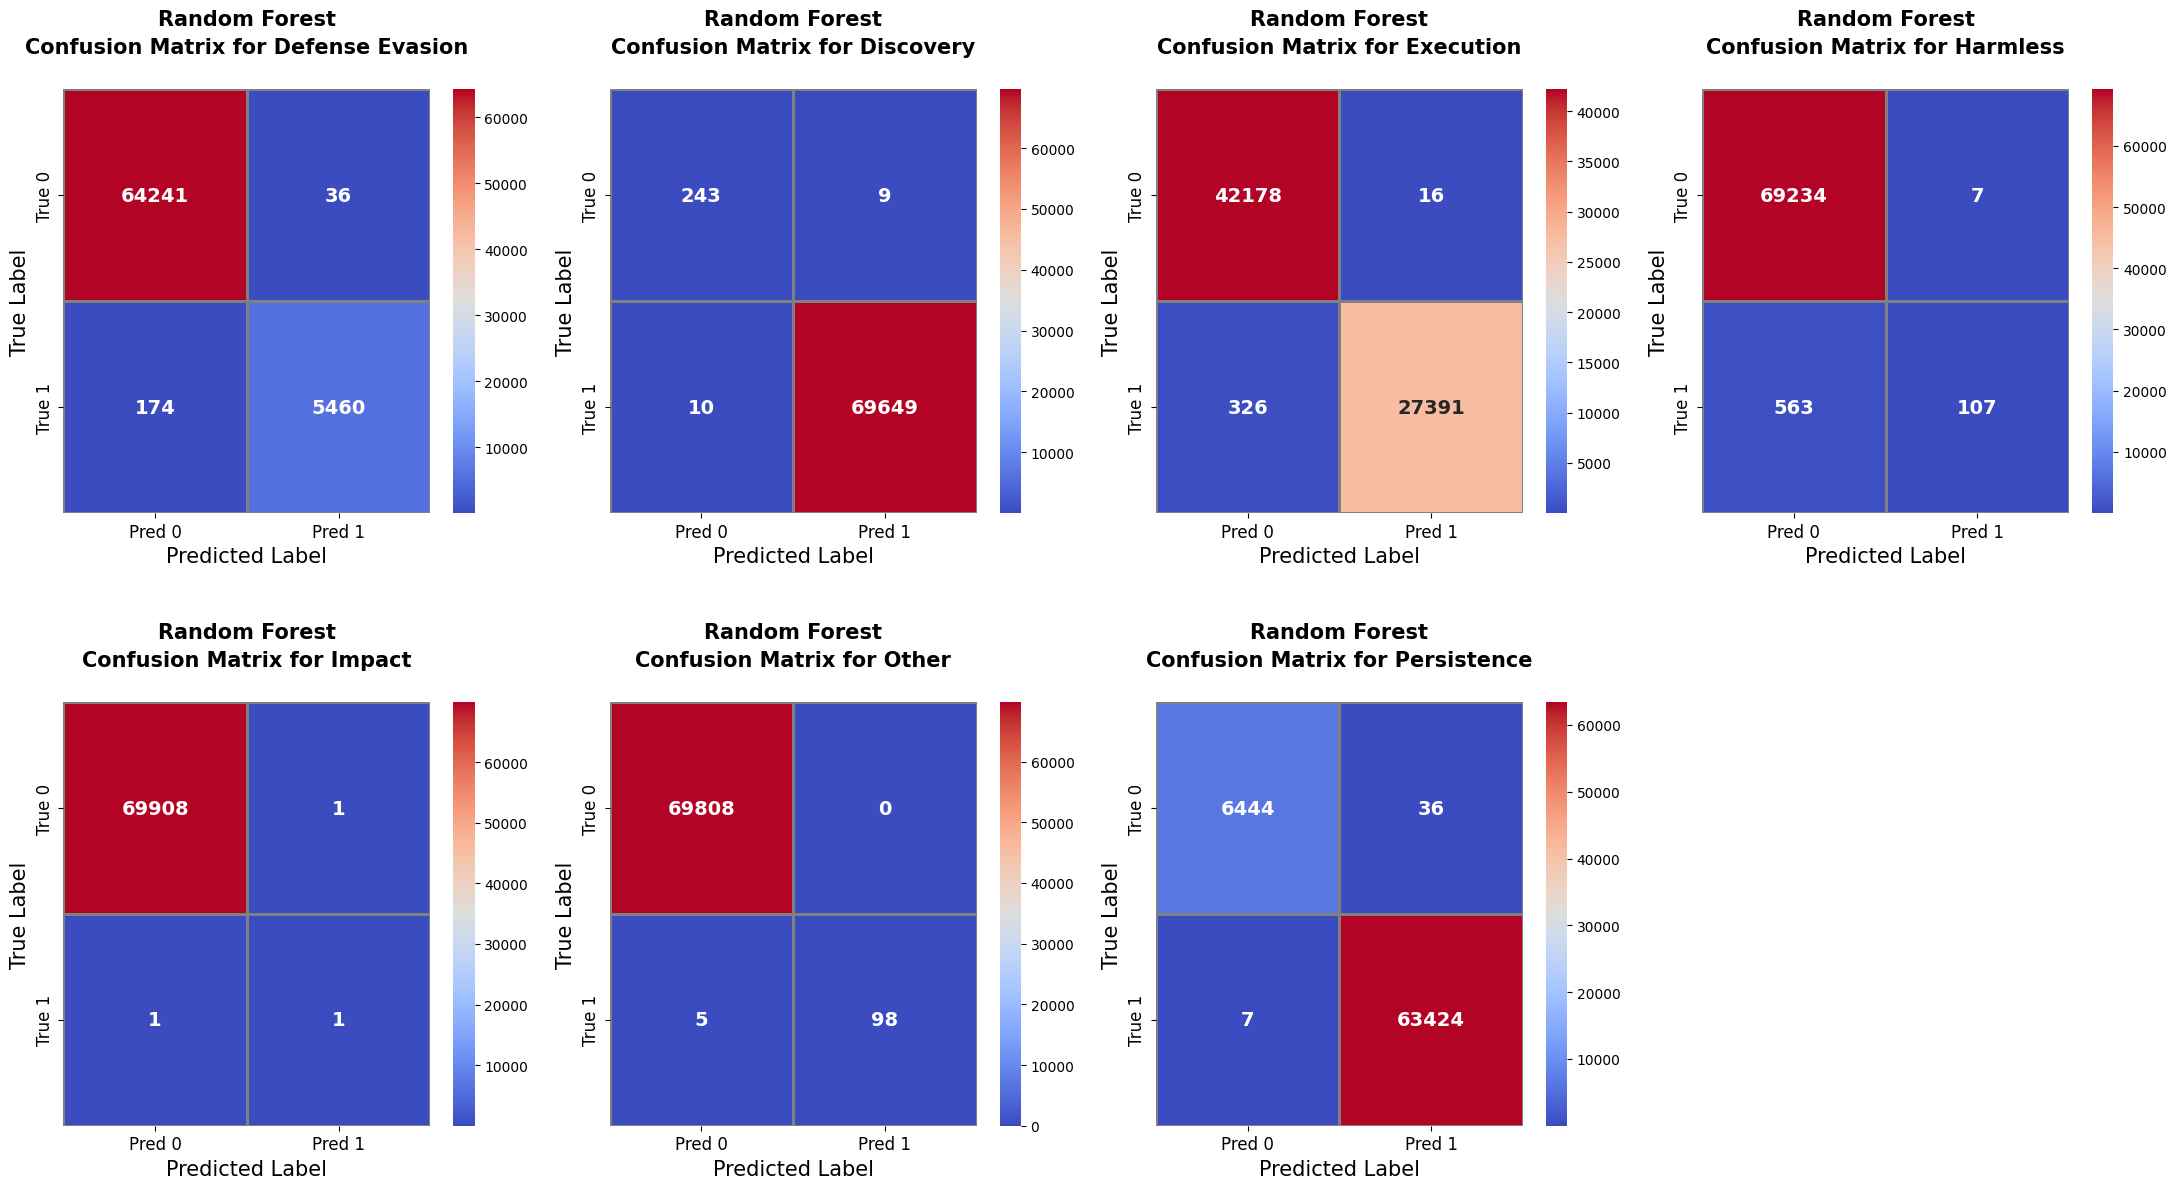
\includegraphics[width=0.77\textwidth]{../figures/plots/section2/Random_Forest_normalized_confusion_matrix_test.png}
                    \caption{Random Forest Confusion Matrices}
                    \label{fig:rf_cm_base}
                \end{minipage}%
            \end{minipage}

            \vspace{0.5cm}  % Add some vertical spacing between rows
            
            % Middle row  
            \begin{minipage}{\textwidth}
                % Middle-left (Train)
                \begin{minipage}[c]{0.48\textwidth}
                    \centering
                    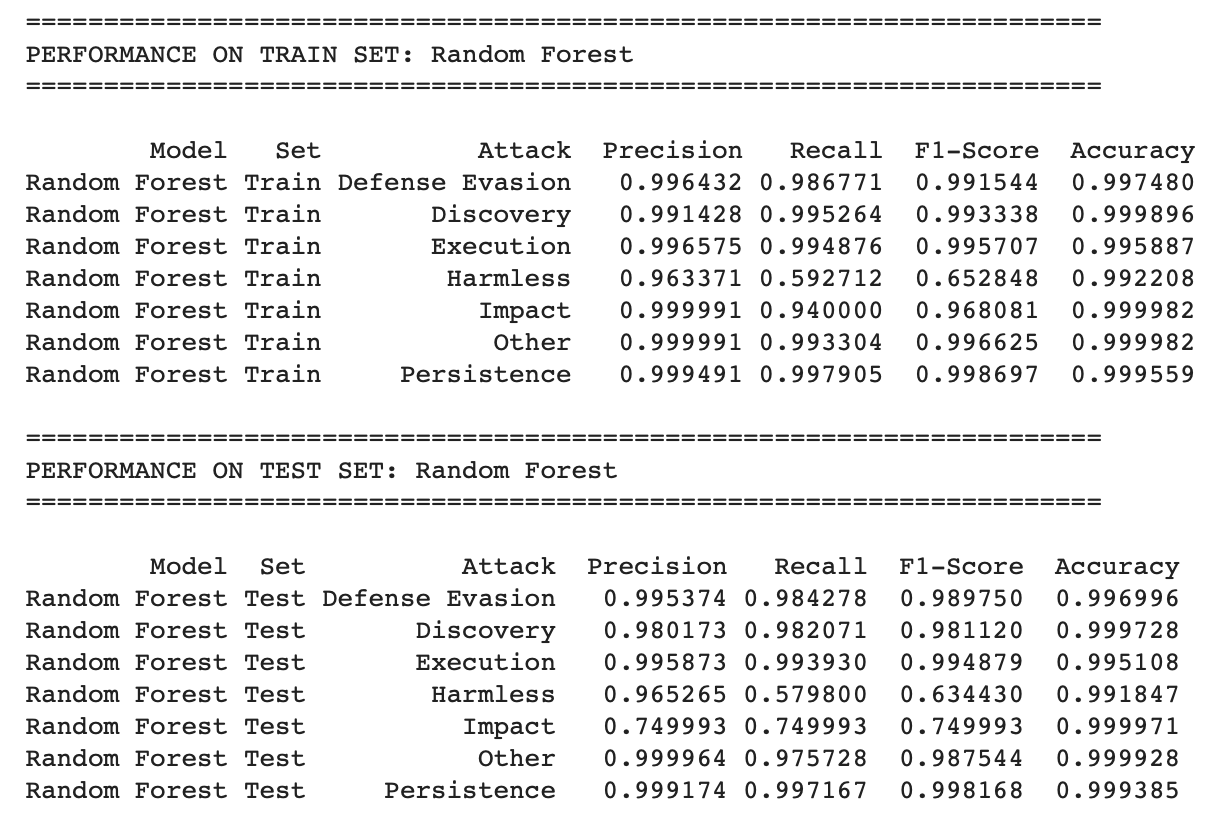
\includegraphics[width=0.9\textwidth]{../figures/plots/section2/Random_Forest_evaluation_metrics.png}
                    \caption{Random Forest Evaluation Metrics}
                    \label{fig:rf_em_base}
                \end{minipage}%
                \hfill%
                % Middle-right (Train)
                \begin{minipage}[c]{0.48\textwidth}
                    \centering
                    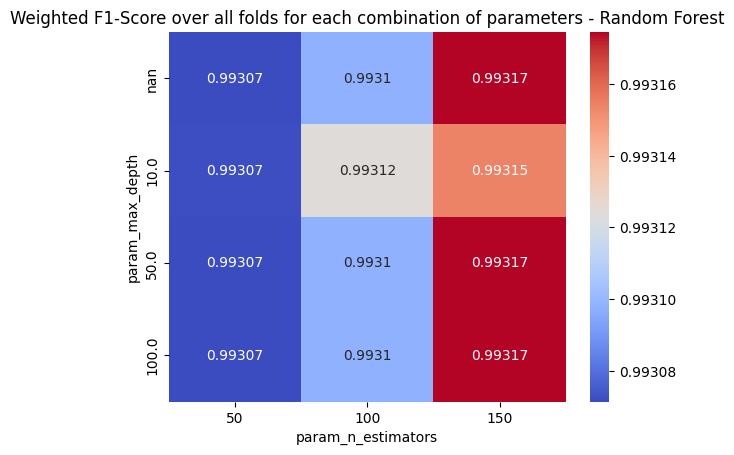
\includegraphics[width=0.7\textwidth]{../figures/plots/section2/weighted_f1_score_for_each_combination_of_parameters_random_forest.png}
                    \caption{Random Forest Weighted F1 Scores}
                    \label{fig:rf_f1_tuning}
                \end{minipage}
            \end{minipage}
            
            \vspace{0.5cm}  % Add some vertical spacing between rows

            % Bottom row
            \begin{minipage}{\textwidth}
                % Bottom-left (Test)
                \begin{minipage}[t]{0.48\textwidth}
                    \centering
                    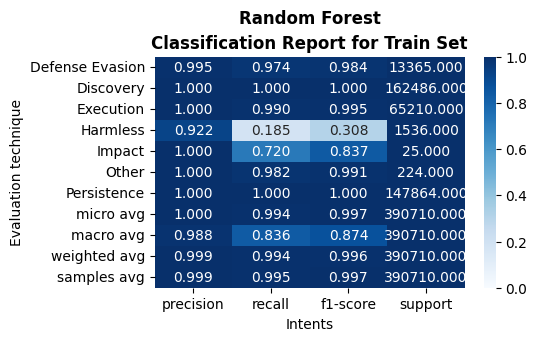
\includegraphics[width=0.9\textwidth]{../figures/plots/section2/Random_Forest_classification_report_for_Train_set.png}
                    \caption{Random Forest Classification Report Train Set}
                    \label{fig:rf_cm_train}
                \end{minipage}%
                \hfill%
                % Bottom-right (Test)
                \begin{minipage}[t]{0.48\textwidth}
                    \centering
                    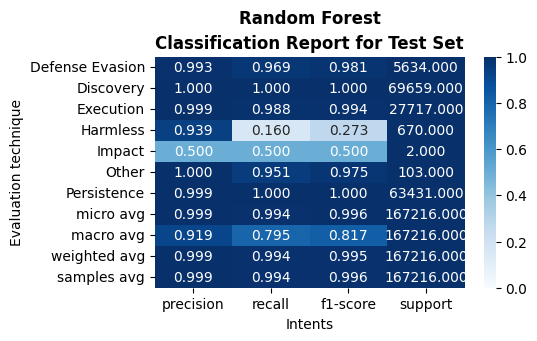
\includegraphics[width=0.9\textwidth]{../figures/plots/section2/Random_Forest_classification_report_for_Test_set.png}
                    \caption{Random Forest Classification Report Test Set}
                    \label{fig:rf_cm_test}
                \end{minipage}  
            
            \end{minipage}
            
        \end{figure}
            
        \clearpage
    
        % SVM
        
        \begin{figure}[H]
        
            \centering
            
            % Top row
            \begin{minipage}{\textwidth}
                \centering
                \begin{minipage}[c]{\textwidth}
                    \centering
                    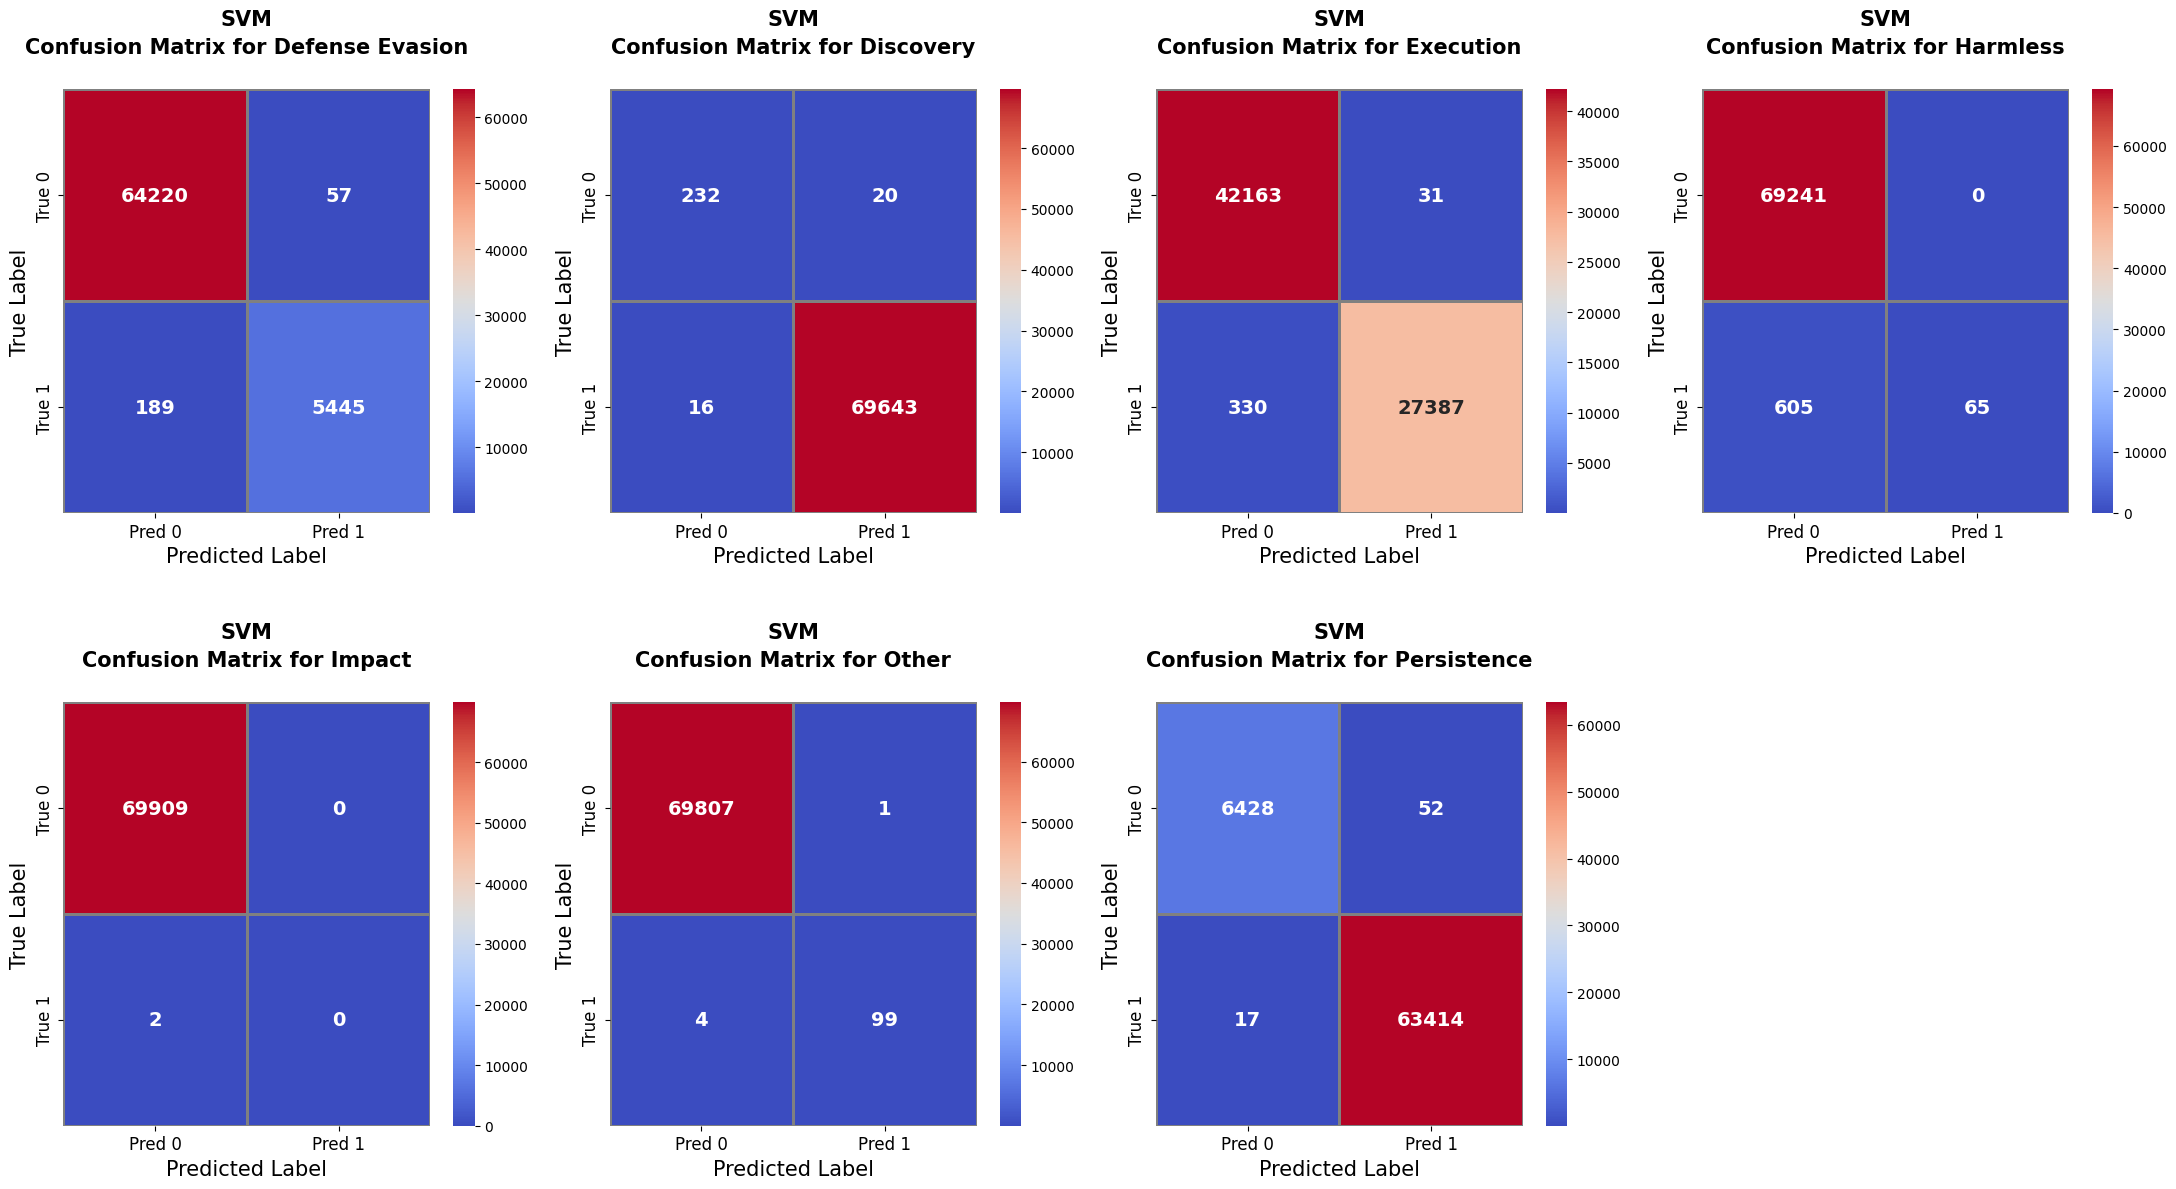
\includegraphics[width=0.77\textwidth]{../figures/plots/section2/SVM_normalized_confusion_matrix_test.png}
                    \caption{SVM Confusion Matrices}
                    \label{fig:svm_cm_base}
                \end{minipage}%
            \end{minipage}

            \vspace{0.5cm}  % Add some vertical spacing between rows
            
            % Middle row  
            \begin{minipage}{\textwidth}
                % Middle-left (Train)
                \begin{minipage}[c]{0.48\textwidth}
                    \centering
                    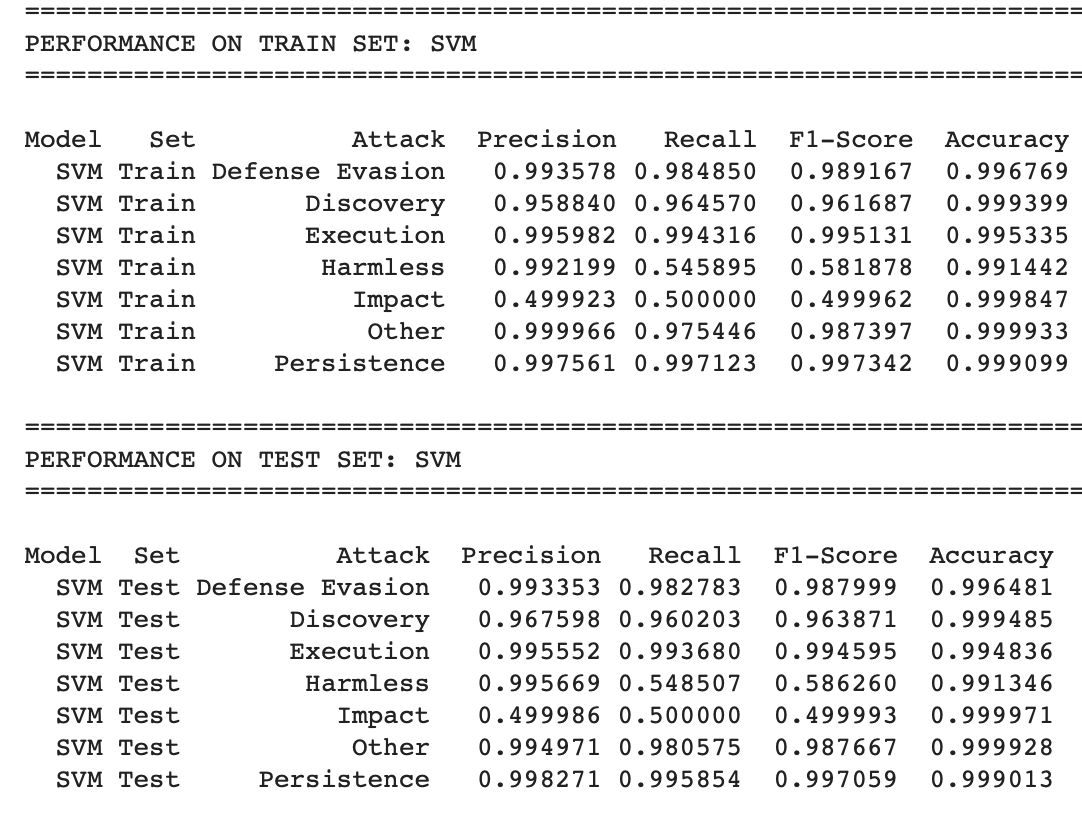
\includegraphics[width=0.8\textwidth]{../figures/plots/section2/SVM_evaluation_metrics.png}
                    \caption{SVM Evaluation Metrics}
                    \label{fig:svm_em_base}
                \end{minipage}%
                \hfill%
                % Middle-right (Train)
                \begin{minipage}[c]{0.48\textwidth}
                    \centering
                    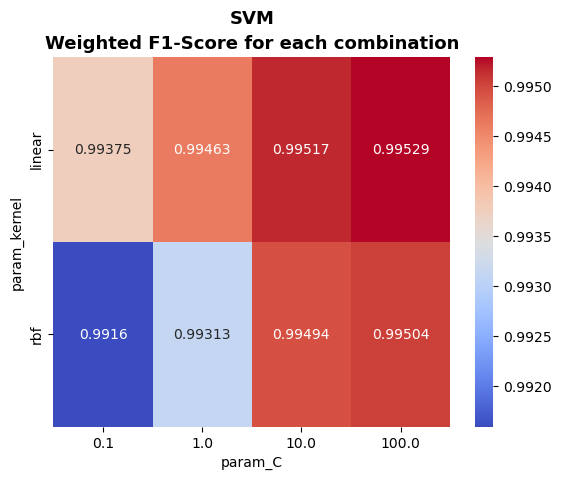
\includegraphics[width=0.7\textwidth]{../figures/plots/section2/weighted_f1_score_for_each_combination_of_parameters_svm.png}
                    \caption{SVM Weighted F1 Scores}
                    \label{fig:svm_f1_tuning}
                \end{minipage}
            \end{minipage}
            
            \vspace{0.5cm}  % Add some vertical spacing between rows

            % Bottom row
            \begin{minipage}{\textwidth}
                % Bottom-left (Test)
                \begin{minipage}[t]{0.48\textwidth}
                    \centering
                    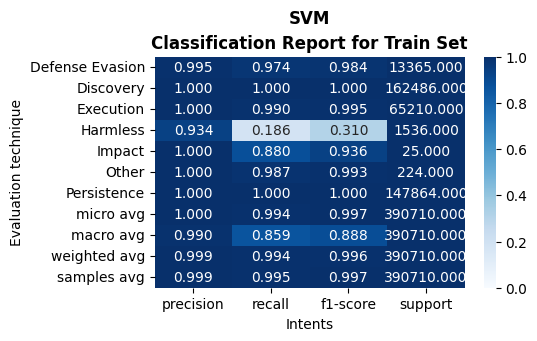
\includegraphics[width=0.9\textwidth]{../figures/plots/section2/SVM_classification_report_for_Train_set.png}
                    \caption{SVM Classification Report Train Set}
                    \label{fig:svm_cm_train}
                \end{minipage}%
                \hfill%
                % Bottom-right (Test)
                \begin{minipage}[t]{0.48\textwidth}
                    \centering
                    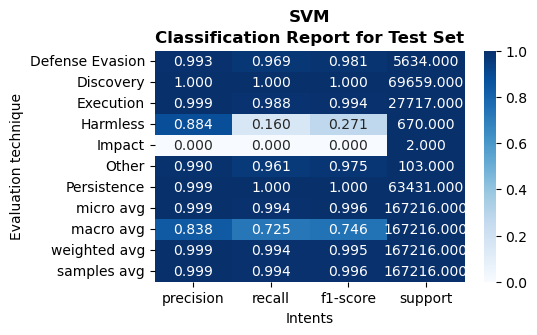
\includegraphics[width=0.9\textwidth]{../figures/plots/section2/SVM_classification_report_for_Test_set.png}
                    \caption{SVM Classification Report Test Set}
                    \label{fig:svm_cm_test}
                \end{minipage}  
            
            \end{minipage}
            
        \end{figure}
